\documentclass[a4paper,12pt]{article} % тип документа
\usepackage[margin=1in]{geometry} % Поля

%  Русский язык
\usepackage[warn]{mathtext}
\usepackage[T2A]{fontenc}			% кодировка
\usepackage[utf8]{inputenc}			% кодировка исходного текста
\usepackage[english,russian]{babel}	% локализация и переносы
% Математика
\usepackage{amsmath,amsfonts,amssymb,amsthm,mathtools} 
\usepackage{wasysym}
%%%
\usepackage{graphicx}

\usepackage{tabularx}

\usepackage{gensymb} % знак градуса
\usepackage{enumitem} % изменить список enumerate
\usepackage{placeins} % \FloatBarrier

\renewcommand{\thesection}{\Roman{section}} 
\renewcommand{\thesubsection}{\roman{subsection}}


\begin{document}

\newcolumntype{Y}{>{\centering\arraybackslash}X} %new tabularx


%титул
\hrule 	
\medskip
\begin{raggedright}
{\large \textbf{Отчёт по работе 4.5.3}}
\\
\medskip
{\Large Сканирующий интерферометр} 
\\
\medskip
{\large Карташов Констанин Б04-005}
\medskip
\hrule
\medskip
\end{raggedright}


\section{Анотация}

\paragraph{Цель работы:} 
Знакомство с устройством и работой газового лазера непрерывного действия, со спектральными характеристиками лазерного излучения, а также с устройством и принципом действия сканирующего интерферометра Фабри-Перо.

\paragraph{Оборудование:}
\begin{itemize}
\renewcommand{\labelitemi}{$\triangleright$}
\itemsep-0.5em
\item He-Ne лазер с блоком питания;
\item сканирующий интерферометр Фабри-Перо;
\item поляроид;
\item пластинка $\lambda/4$;
\item линза;
\item фотодиод;
\item электронный осциллограф.
\end{itemize}


\medskip\hrule\medskip

\FloatBarrier

\section{Теоретическая часть}

\subsection{He-Ne лазер}

\paragraph{} He-Ne лазер представляет из себя активную среду в виде колбы заполненной гелием и неоном в соотношении 10:1, в которой гелий используется для накачки неона до уровня излучающего свет с длиной волны $\lambda = 632.8$ нм. И оптический резонатор в виде интерферометра Фабри-Перо.

\paragraph{} Видимый спектр лазера расширяется эффектом Доплера за счёт теплового движения атомов Неона. Частота излучения движущегося источника сдвинута относительно неподвижного источника, в нерелятивистском случае:

\[
\frac{\omega_D}{\omega} \sim \frac{v}{c}\cos{\alpha},
\]

\noindent где $\alpha$ -- угол между вектором скорости направлением на наблюдателя. При хаотическом движении полуширина линии приблизительно составляет:

\[
\Delta \omega_d \sim \omega \frac{v_T}{c} = \frac{\omega}{c}\sqrt{\frac{8k_\text{Б}T}{\pi m}}.
\]

\paragraph{} Оптический резонатор обеспечивает возможность многократного прохождения продольной волны. Большое количество энергии накапливается в виде стоячих волн. На длине резонатора укладывается целое число полуволн. Пики в спектре вызванные собственными частотами резонатора называются собственными модами. Межмодовое расстояние определяется длиной резонатора:

\begin{equation}
\nu_{m+1} - \nu_{n} = \frac{c}{2L}.
\label{modes}
\end{equation}

\subsection{Сканирующий интерферометр Фабри-Перо}

\begin{figure}
\centering
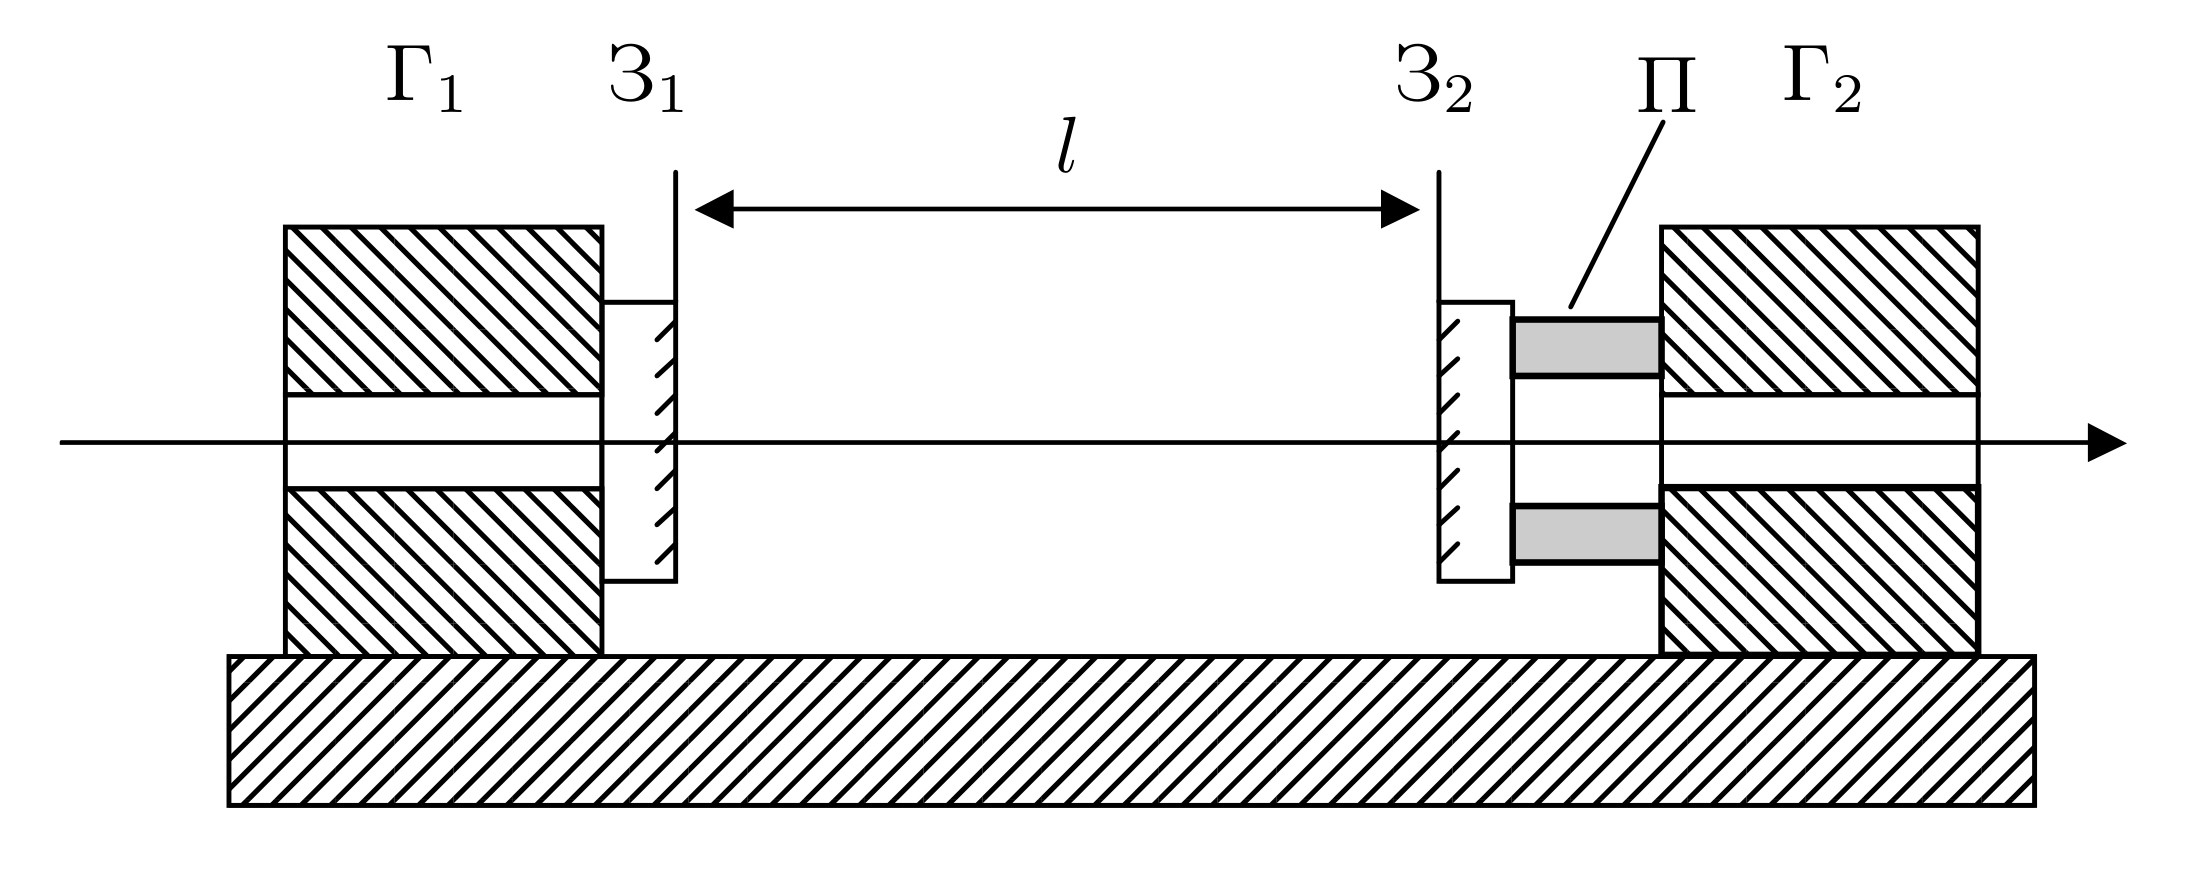
\includegraphics[width=0.7\textwidth]{interf.jpg}
\caption{Устройство сканирующего интерферометра}
\label{interf}
\end{figure}

\paragraph{} Сканирующий интерферометр представляет собой высокодобротный интерферометр Фабри-Перо с периодически изменяемой базой. Его устройство схематически представлено на рис. \ref{interf}. 
\paragraph{} На жёстком массивном основании расположены две юстировочные головки Г$_1$  и Г$_2$, на который укреплены зеркала З$_1$ и З$_2$ соответственно. Зеркало З$_2$ связанно с головкой Г$_1$ через пьезокерамический элемент П.
\paragraph{} Пьезокерамический элемент позволяет периодически изменять базу интерферометра на величину порядка длины световой волны. Элемент имеет форму полого цилиндра. Его внутренняя и наружная поверхности металлизированы и образуют цилиндрический конденсатор. Необходимое изменение длины цилиндра возникает при подаче напряжения в несколько сотен вольт.
\paragraph{} Если вдоль оси интерферометра распространяется световое излучение с длиной вольны $\lambda$, то при выполнении условия
\begin{equation}
2l = m\lambda, \;\;\; m \in \mathbb{N}
\label{e:inter}
\end{equation}

\noindent возникает резонанс. Излучение с такой частотой полностью проходит через интерферометр. Собственные моды интерферометра различаются на частоту:
\[ \Delta \nu = \frac{c}{2L}.
\]

\noindent Величина $\Delta \nu$ называется дисперсионной областью спектрального прибора. В единицах $\lambda$ дисперсионная область сканирующего интерферометра равна
\begin{equation}
\Delta \lambda_\text{СИ} = \frac{\lambda}{m} = \frac{\lambda^2}{2l}.
\label{e:area}
\end{equation}

\paragraph{} Разрешающая способность спектрального прибора определяется отношением:
\begin{equation}
R = \frac{\lambda}{\delta \lambda},
\label{e:res}
\end{equation}

\noindent где - $\delta \lambda$ -- минимальная разность длин волн, разрешаемая прибором вблизи длины волны $\lambda$. Разрешающая способность интерферометра зависит от длины интерферометра $l$ и коэффициента отражения зеркал $r$:
\begin{equation}
R = \frac{2\pi l}{\lambda ( 1 - r )}.
\label{e:res2}
\end{equation}

\medskip\hrule\medskip

\FloatBarrier 

\section{Экспериментальная часть}

\subsection{Устройство экспериментальной установки}

\begin{figure}
\centering
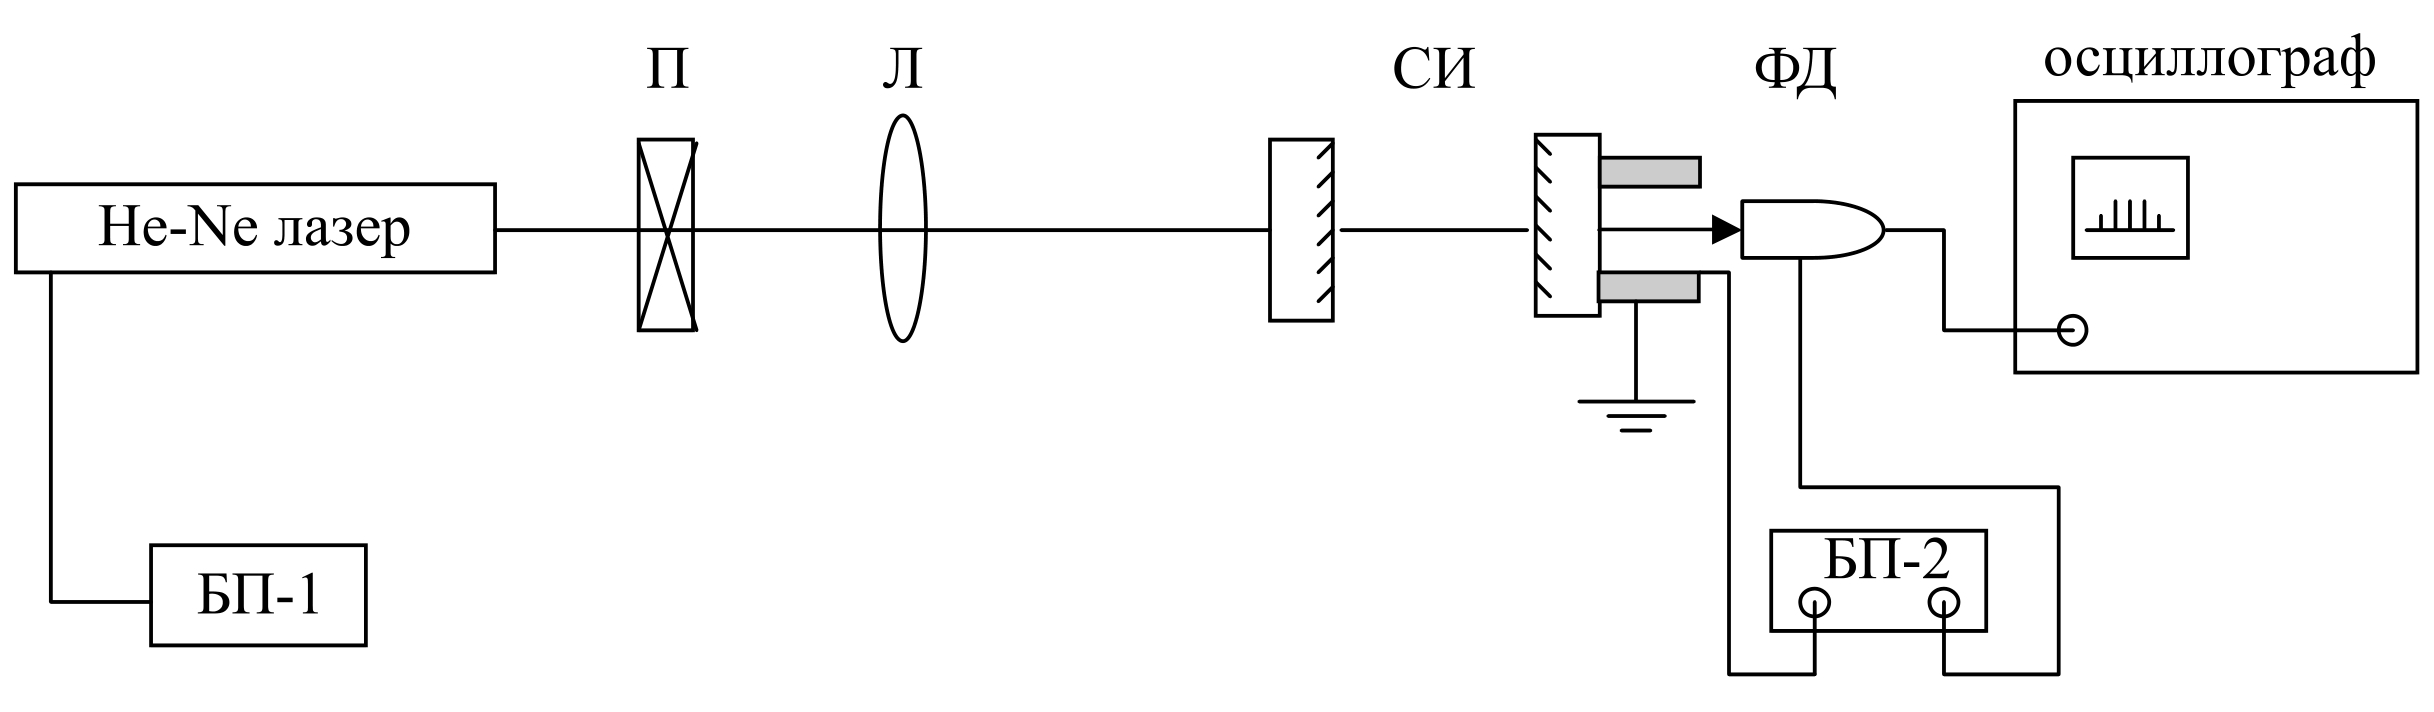
\includegraphics[width=0.9\textwidth]{setup.jpg}
\caption{Схема установки для изучения спектрального состава излучения лазера}
\label{setup}
\end{figure}

Излучение He-Ne лазера проходит через поляризационную развязку П и линзу Л и поступает на вход сканирующего интерферометра (СИ). Поляризационная развязка предотвращает попадание в лазер излучения, отразившегося от элементов оптического тракта. Развязка состоит из поляроида и пластинка $\lambda/4$, главные направления которой установлены под углом 45\degree по отношению к разрешённому направлению поляроида. После развязки П свет приобретает циркулярную поляризацию. При отражении от более оптически плотной среды такой свет приобретёт поляризацию обратную изначальной. Отражённый свет при прохождении через пластинку снова приобретёт линейную поляризацию, однако направление поляризации будет перпендикулярно разрешённому направлению поляроида, поэтому отражённая волна не проходит.

Линза Л служит для уменьшения круга, поступающего на вход сканирующего интерферометра. Линза снабжена поперечными и продольными салазками для юстировки прибора на максимум сигнала.

Излучение прошедшее сканирующий интерферометр, поступает на фотодиод ФД. Напряжения с фотодиода через усилитель подаётся на вертикальный вход электронного осциллографа ЭО. 

Лазер питается от блока питания БП-1, фотодиод и усилитель от БП-2. Напряжение на пьезоэлементе сканирующего интерферометра подаётся с блока питания БП-2 и регулируется ручкой 1.

\paragraph{Параметры установки:}
\begin{itemize}
\renewcommand{\labelitemi}{$\triangleright$}
\itemsep0em
\item Длина лазера $L = 65$ см.
\item Длина волны лазера $\lambda = 632,8$ нм.
\item Длина интерферометра $l = 9$ см.
\end{itemize}

\subsection{Задание}

\paragraph{} Откалибруем установку. Для этого совместим лучи в интерферометре, настроим поляризационную развязку, сфокусируем пучок при помощи линзы и совместим ость фотодиода с лучом. Получим устойчивую осциллограмму (рис. \ref{osc}).

\begin{figure}
\centering
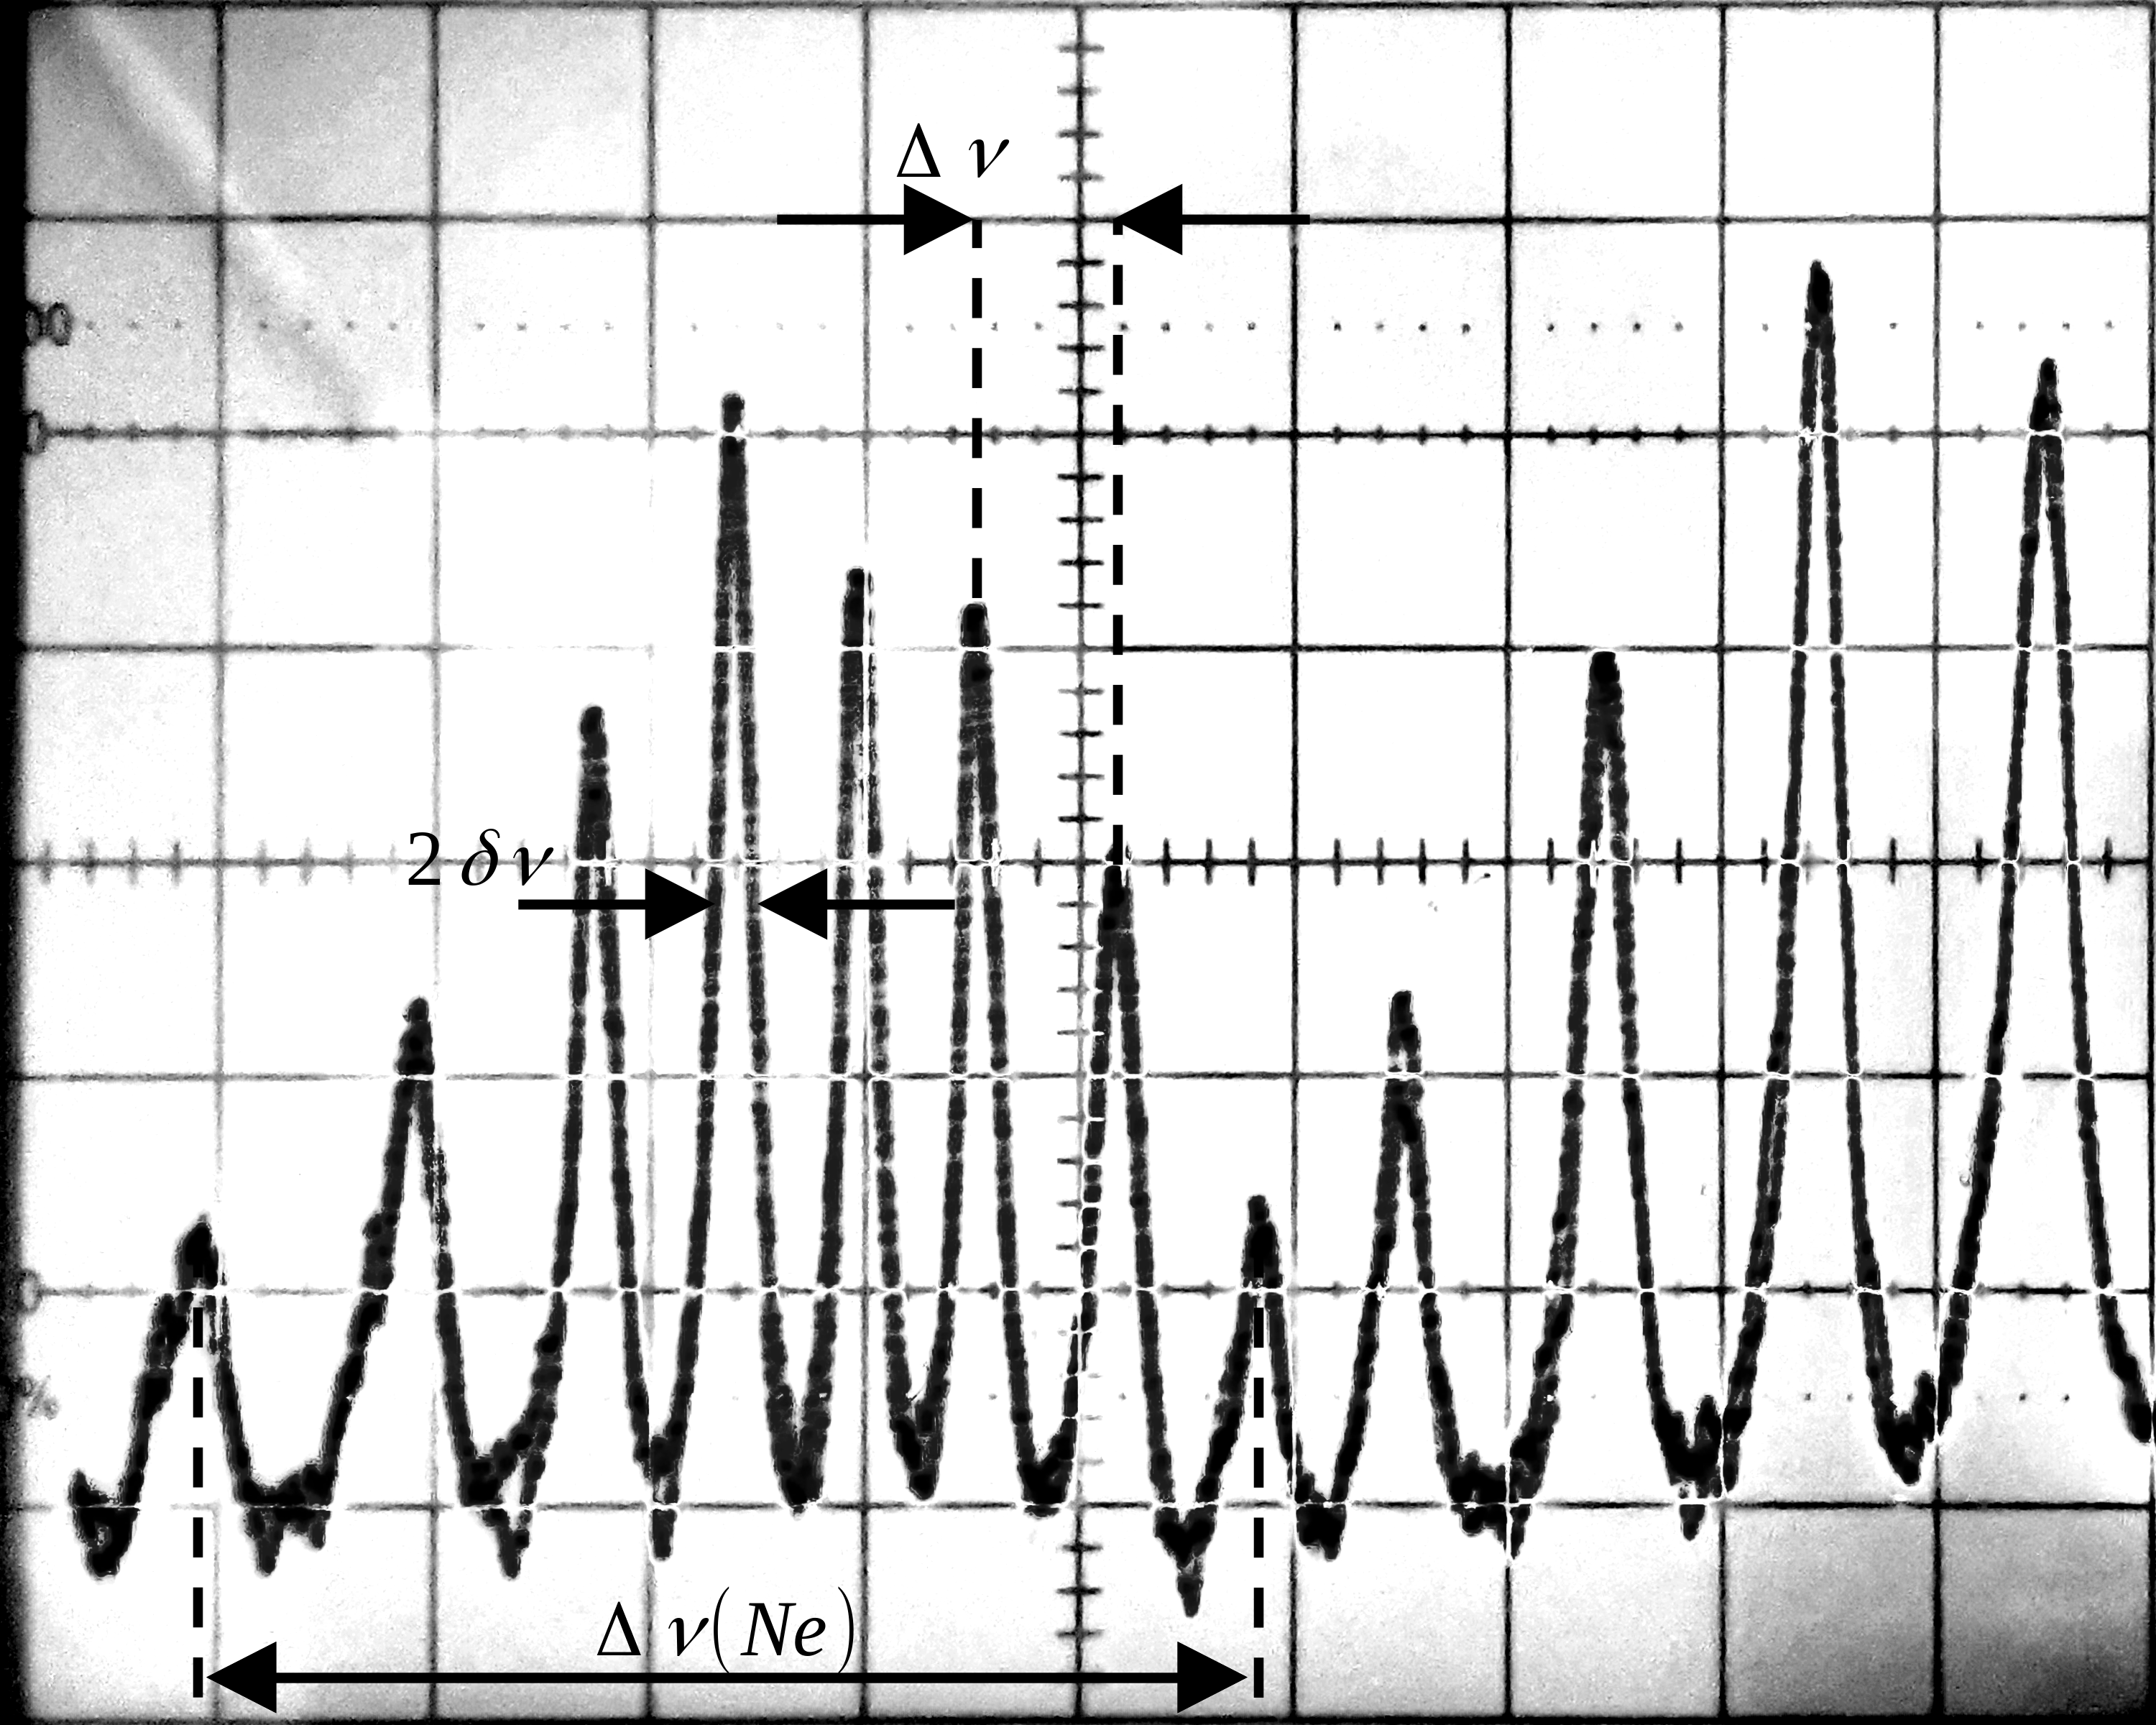
\includegraphics[width=10cm]{osc2.png}
\caption{Осциллограмма спектральной линии}
\label{osc}
\end{figure}

\paragraph{} Рассчитаем межмодовое расстояние лазера в единицах $\nu$ и $\lambda$ по формуле (\ref{modes}). Получим:

\[
\Delta \nu = \frac{c}{2L} = \frac{c}{1.3 \; \text{м}} \approx 231 \; \text{МГц}, 
\]\[
\nu = \frac{c}{\lambda} \approx 4.7376 \cdot 10^14 \; \text{Гц},
\]\[
\Delta \lambda = \lambda \frac{\Delta \nu}{\nu} = \frac{\lambda^2}{c} \Delta \nu = \frac{\lambda^2}{2 L} = \frac{(632.8 \cdot 10^{-9})^2}{1.3} \approx 3.08 \cdot 10^{-13} \; \text{м}.
\]

\noindent Итого: $\Delta \nu = 231$ МГц, $\Delta \lambda = 3.08 \cdot 10^{-13}$ м.

\paragraph{} Сосчитав число промежутков между модами на осциллографе, оценим видимую ширину спектральной линии неона $\Delta \nu (\text{Ne})$. Число промежутков $n = 6$, получим:
\[
\Delta \nu (\text{Ne}) = 6 \Delta \nu \approx 1.38 \; \text{ГГц},
\]\[
\Delta \lambda (\text{Ne}) = 6 \Delta \lambda \approx 18.4 \cdot 10^{-13} \; \text{м}.
\]

\paragraph{} Пологая, что ширина спектральной линии обусловлена эффектом Доплера и, что видимая ширина линии неона порядка полуширины доплеровского контура ($2 \Delta \lambda_D \approx \Delta \lambda (\text{Ne})$. Оценим среднею скорость атомов неона $v_x$ и газокинетическую температуру $T$ в разряде по формуле:
\begin{equation}
\frac{\Delta \lambda_D}{\lambda} = \frac{\Delta \nu_D}{\nu} \approx \frac{v_x}{c}; \;\;\;
\frac{mv_x^2}{2} = \approx \frac{kT}{2}.
\end{equation}
Получаем:
\[v_x \approx c \frac{\Delta \nu_d}{\nu} = c \frac{\Delta \nu (\text{Ne})}{2\nu} = c \frac{0.69 \cdot 10^9}{4.737 \cdot 10^{14}} = c \cdot 3.42 \cdot 10^{-6} \approx 437 \; \text{м/с},
\]\[
T \approx \frac{mv_x^2}{2} = \frac{3.3532 \cdot 10^{-26} \cdot 437^2}{1.38 \cdot 10} \approx 464 \; \text{К}.
\]

\paragraph{} Рассчитаем дисперсионную область $\Delta \lambda_\text{СИ}$ по формуле (\ref{e:inter}) и сравним её с шириной линии неона ($\Delta \lambda (\text{Ne})$):
\[
\Delta \lambda_\text{СИ} = \frac{\lambda^2}{2l} = \frac{(632.8 \cdot 10^{-9})^2}{2 \cdot 0.09} \approx 2.2 \cdot 10^{-12} \; \text{м}.
\]
\noindent Ранее полученное значение $\Delta \lambda (\text{Ne}) \approx 1.8 \cdot 10^{-12}$ очень близко к этому значению.

\paragraph{} Сравним ширину отдельной моды на полувысоте с межмодовым расстоянием, и оценим разрешающую способность $R$ по формуле (\ref{e:res}). По осциллограмме получаем, что $2\delta \nu = 0.2$ деления на экране осциллографа, $\Delta \nu = 0.65 $ деления, получаем:
\[
\delta \nu = \frac{0.1}{0.65} \Delta \nu = 0.15 \cdot 3.08 \cdot 10^{-13} \approx 0.5 \cdot 10^{-13} \; \text{м},
\]\[
R = \frac{\lambda}{\delta \lambda} = \frac{•}{•}.3 \cdot 10^{-7}}{5 \cdot 10^{-14}} \approx 10^{7}. 
\]

\paragraph{} Оценим коэффициент отражения $r$ по формуле (\ref{e:res2}):
\[
r = 1 - \frac{2\pi l}{\lambda R} = \frac{2 \pi \cdot 0.09}{6.3 \cdot 10^{-7} \cdot 10^{7}} \approx 0.91.
\] 

\medskip\hrule\medskip

\section{Выводы}

\begin{enumerate}
\item Настроив экспериментальную установку, мы получили устойчивое изображение спектральной линии с видимыми на ней собственными модами лазера и его доплеровским контуром.
\item Изучив спектральную линию нашли примерную скорость и температуру молекул в лазере: $v_x 	\sim 440$ м/с, $T \sim 450$ К.
\item Изучив спектральную линию определили разрешающую способность интерферометра $R \approx 10^7$ и коэффициент отражения зеркал $r \approx 0.91$.
\end{enumerate}

\medskip\hrule\medskip

\end{document}
